%----------------------------------------------
%%% LSOP...
\section{Appendix: Laser Standard Operation Procedure}
\label{sec:lsop}

\subsection{ Introduction}

A polarized $^3$He target system was built and used for several 
JLab experiments. A number of new experiments will continue use the 
polarized $^3$He target system in the future. 
The polarized $^3$He target is based on 
the principle of spin exchange between optically pumped Rubidium vapor and 
$^3$He gas. Several high power (30 Watts) 795 nm diode lasers will be used 
for the optical pumping. A laser hut has been built and installed in Hall A.
This LSOP describes the setup of the 
laser system in the laser hut and at the target area, 
details the potential
hazards associated with the operation of this setup and provides instructions
for the safe and effective use of the equipment. In addition,
this manual provides information about the functioning of the various safety 
systems installed to protect personnel and equipment.

\subsection{Personnel}

The 30 watts infrared diode lasers (Coherent FAP-System) may only be operated by
personnel who have :
\begin {itemize}
\item completed a Laser Safety course administrated by the laser safety officers at
Jefferson Laboratory (Patty Hunt).
\item read the Laser Safety section of the EH\&S Manual(6410);
\item  completed and passed an opthalmological exam;
\item had a safety walkthrough by the Laser Safety Supervisor of the 
Polarized $^3$He Target System (Jian-ping Chen);
\item read this document;
\item been added to the authorized list of Laser Personnel, included as the 
last page of this LSOP.
\end {itemize}
Jefferson Lab personnel or outside visitors, who have not completed all of 
above training, are
only allowed to enter the laser control area under the following conditions :
\begin {itemize}
\item have permission of the Laser Safety
Supervisor of the Polarized $^3$He target system
\item be accompanied by a laser authorized personnel
\item if the laser is operational, with required safety
goggles
\item if any equipment, including the laser, is operational, no touching of
equipment due to electrical hazards.
\end {itemize}


\subsection{Laser}

The main Laser specifications are outlined in Table 1. For more specific
information, we refer to the Coherent FAP-system diode laser users manual, 
which will be available in the lab.

\begin{table}
\begin{center}
\begin{tabular}{|l|l|}
\hline
& \\
{\bf Specifications}&{\bf COHERENT FAP-System} \\
\hline
& \\
\underline {\it Operational Specifications}& \\
Output power			& 30 W \\
& \\
\underline {\it Mechanical Specifications}& \\
Weight			        & 60 pounds  \\
Cooling Requirements 		& None required \\
Delivery Optical Fiber Bundle   & 0.8 mm diameter \\
Delivery Fiber Length		& 5.0 meter nom.\\
Delivery Fiber Termination	& SMA 905 conn. \\
& \\
\underline {\it Operational Specifications}& \\
Typical Operating Temperature   & $0^\circ$C to $35^\circ$C \\
Typical Storage Temperature     & $-20^\circ$C to $65^\circ$C \\
Humidity (non-condensing)       & $5\%$ to $95\%$  \\
& \\
\underline {\it Electrical Specifications}& \\
Input Power	                & 115 Vac 60 Hz, $<1200$ W (500 W typical) \\
& \\
\underline {\it Optical Specifications}& \\
Beam Characteristic 		& Semiconductor, multimode \\
Beam Divergence        & $<0.20$ N. A. \\
Diode Laser Center Wavelength   & 780 to 840 nm \\
Wavelength Temp Coefficient	& 0.27 to 0.30 nm/$^\circ$C \\
Emission Bandwidth (FWHM)       & $\pm 2$ nm \\
\hline
\end{tabular}
\label{speclaser}
\caption{Laser specifications}
\end{center}
\end{table}


\subsection{Optical setup}

The optical setup is shown in Fig.~\ref{fig:laser_setup}, and is made of:
\begin {itemize}
\item A optical table (stainless steel) supporting one breadboard 
(anodized aluminum);
\item Seven infra-red diode lasers (four for longitudinal pumping and three 
for transverse pumping) located on one side of the table, with optical 
fiber bundles.
\item Seven lens to have each laser beam focused at the pumping cell;
\item Seven beam splitters to split each laser beam to two beams;
\item Fourteen $\lambda$/4 waveplates to transform each beam from
linear polarization to right or left circular polarization;
\item Fourteen dielectric mirrors to reflect each split beam back into the pumping cell;
\item One transparent window on the RF enclosure and one transparent window 
on the oven to allow the combined transverse laser beam to pass through;
\item Two dielectric mirrors to reflect the combined longitudinal 
laser beam into the pumping cell;
\item One pumping cell to absorb all the laser beam power;
\item Three mirrors for monitoring the pumping cell;
\item One spectral-analyzer for monitoring the pumping cell.
\end {itemize}

The optical table will be about 2 meters from the platform.
The laser beams will be from about 15 cm to 105 cm above the table
Each of the 795 nm diode laser light, after passing through the lens,
will be split into two beams. Each one will go through a $\lambda$/4 waveplate
to transform linear polarization to circularly right or left polarization. 
All beams, after passing some windows and being reflected by some mirrors,  
will shoot into a glass pumping cell filled with
mixture of Rb vapor and $^3$He gas. The laser beams will be completely absorbed
by the pumping cell. The total path length from the lasers to the pumping cell
is about 5 meters. The pumping cell is inside an oven and 
connected to a target cell. The whole target assembly is inside two pairs of
Helmholtz coils, which provide a magnetic field for the polarization of the
target. A NMR system with a set of RF drive coils and a set of separate 
pickup coils, and an EPR system 
are used to measure the polarization of the target.


\subsection{Hazards}

The primary beam hazards associated with Class IV lasers consists of eye and skin
injuries. The most severe eye injuries are caused by viewing the beam either directly
or through specular reflection. At an infra-red wavelength of $795 nm$ most of the
laser light entering the eye is absorbed in the retina. The primary adverse effects
from direct or specular viewing are blindness and severe retinal burns. The primary
adverse effects from accidental viewing are retinal burns. The retina is most
sensitive to radiation of this wavelength, and if the laser energy incident to the eye
is too high, it can cause an irreversible retinal burn.

Laser radiation of the intensity associated with Class IV diode lasers can also
cause irreversible damage to the skin. The damage caused is either associated with
temperature rise of the skin tissue following the absorption of laser energy (skin
burns) or with surface reactions resulting from photon interactions at the molecular
level (photochemical effect), disrupting the normal functionality of the skin tissue.

The normal Hazard Zone for the 30 Watts FAP system is $2.76 \times 10^3$ meters.


\subsection{Laser environment}

The diode lasers and the associated devices will be located in the polarized $^3$He target laser hut in Hall A.
The entire hut is a laser controlled area. Its organization is shown in
Fig.\ref{fig:laser_hall}. The setup will be on the second floor and the direct laser light
will not be visible from the entrance of the room.


\begin{figure}
%  \begin{center}
  \centerline{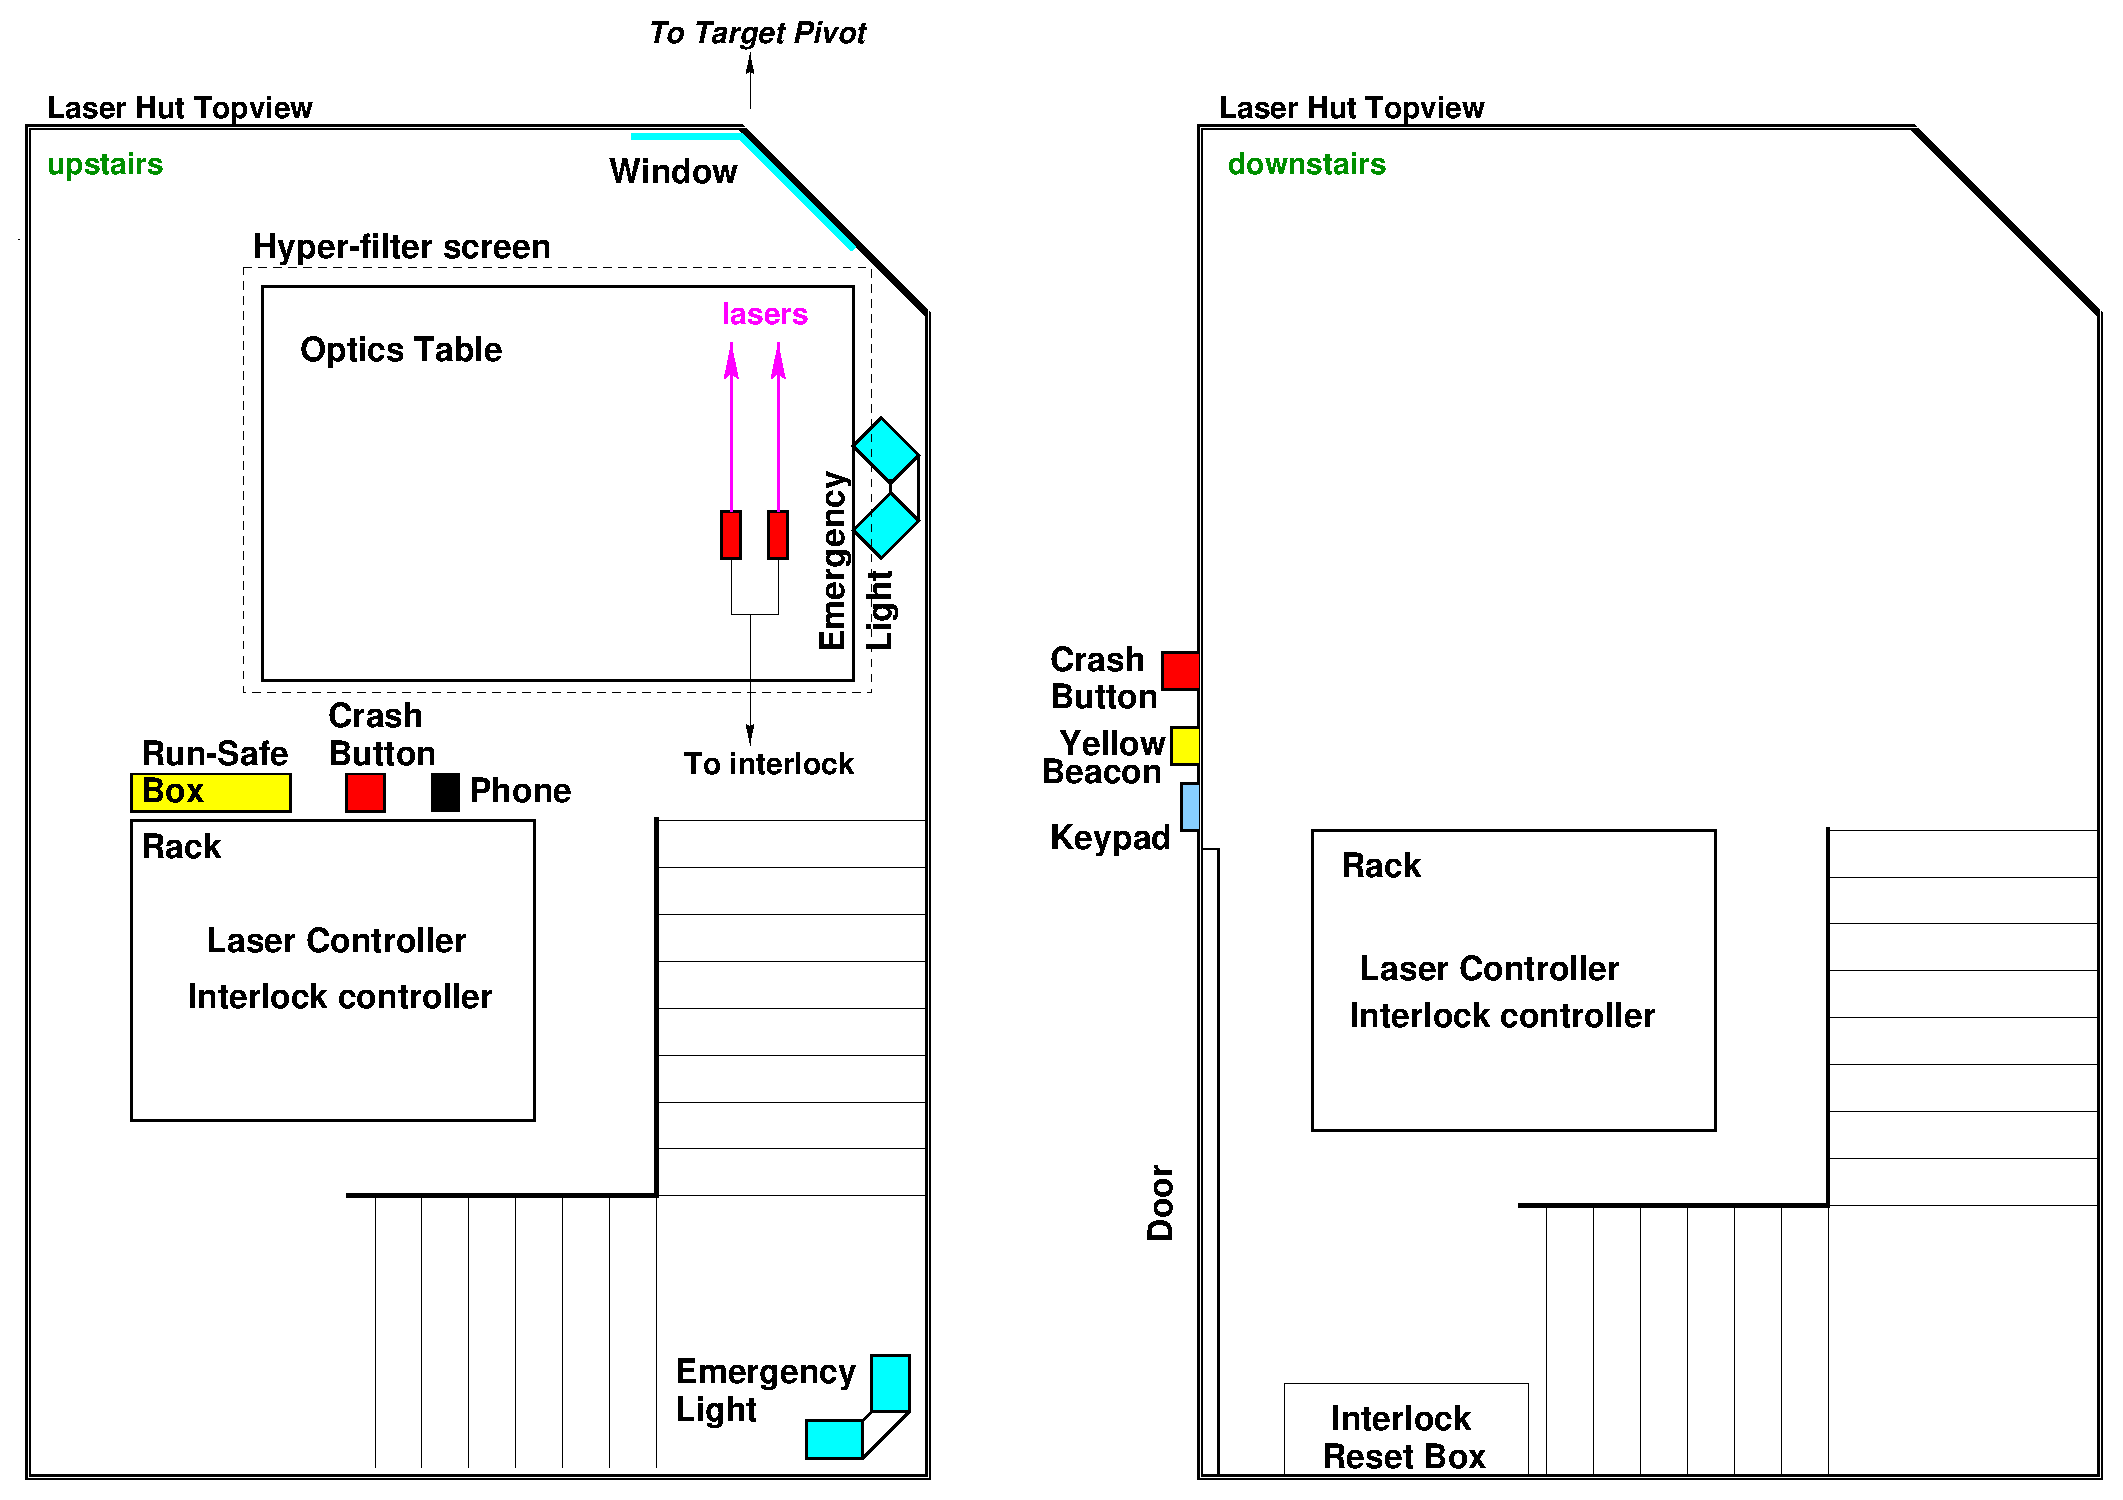
\includegraphics[height=\textwidth]{laser_hall}}
  \caption[Polarized $^3$He Laser Hut]{The Polarized $^3$He Target Laser Hut Setup}
%  \end{center}
   \label{fig:laser_hall} 
\end{figure}

The laser beams are horizontal and are pointing away from the entrance door. 
After passing through the optical setup, the laser beams 
are directed into the pumping cell and terminated there. 

Outside the laser hut, the laser beam path is completely enclosed with beam 
pipe between the laser hut and the target pivot and an enclosure on top of the 
the target. 
Since the beam path is not enclosed inside the laser hut, any partially
reflective surface may cause deflection of the beam path. When operating the 
diode laser, safety goggles are required at all times.  

Apart from direct beam hazards to eyes and skin, since the diode lasers are 
Class IV lasers, there exists a potential fire hazard. Flammable material 
should not be brought into the laser area.  

\subsection{Procedures}

In this section, we review the various procedures that are required to operate the
laser and optical devices. Hazards are least likely to occur during normal operation
when laser beams are switched on. During tests, maintenance,
upgrades and/or alignment,  beam hazards are more likely.

{\bf At all times}, when operating the diode lasers in lasing mode, safety goggles
are required.

\subsubsection{Normal procedure}
In the operation mode, each diode laser is in lasing mode rendering an output 
power of approximately 30 W. The laser beam is already aligned, properly 
focused and directed into the pumping cell. The lasers are interlocked with the
entrance door of the laser hut. All the laser beam pipes and the laser 
enclosure on top of the target are securely installed.

Working with the lasers in normal operational mode will require protective 
eye wear with a minimum optical 
density (OD) of 4.7 at wavelength of 795 nm. Before
starting the laser in its normal operation mode personnel have to enable the
laser safety interlock box. This will cause access to the laser hut to be in 
a controlled mode. Authorized personnel with an access code can 
bypass the interlock for 45 seconds when entering the laser room. Unauthorized
personnel entering the room will cause the lasers switching to stand-by mode
when the door is opened. If the laser is to be unattended for a long time, the 
power should be switched off.

Thus the general procedures for normal operation of the diode lasers in the target lab are:

\begin {itemize}
\item Enable laser safety interlock box;;
\item Wear protective eyewear;
\item Switch on AC power;
\item Turn on the control box with a key; 
\item Turn laser to Ready and then On.
\end {itemize}

\subsubsection{Alignment procedure}

All the mechanical stands supporting the optical components have been designed and
surveyed in order to achieve a preliminary safe alignment of the entire setup (laser
off).  Initial setup of laser and optical system will be done while the laser 
hut window is closed (such that no laser beam will come out the laser hut).
Initial alignment will be done with a standard class 3 HeNe laser  
(class 3A after attenuation, 650 nm) or a laser pointer (class 3A).
 Laser safety goggles are mandatory for all procedures except for alignment
 using class 3A HeNe laser. Use precaution for class 3A laser when using the 
HeNe laser: Do not look directly into the beam or use collecting optics.
The final alignment will be done with the diode laser but at a reduced laser power (less than 10 amps, when the laser spot on a card can be clearly
seen with IR viewer). The alignment is performed with one laser beam line at a time. 
The beam can be tracked by the use of either an IR viewing card or
an IR viewer.  The photosensitive card can be displaced along the beam, and
the IR viewer allows the tracking by the light slightly diffused on the optical
components. During this final alignment, the laser hut window will be opened 
and the laser beam will be directed to the target, while the laser beam pipes 
and the laser enclosure on top of the target will be taken off. Therefore the 
whole hall will be classified as laser area. We will use the CANS system
to have controlled access. Before the laser alignment starts, a sweep will
be performed to clear the Hall. Then the CANS system will be programmed to
only allow authorized laser trained persons to have access to the hall.   
The door to the BSY tunnel will be magnetically locked with a toggle push-button switch. The ``laser danger'' warning sign will be posted at all the entrances. The doors will be checked by pulling the door handle. In addition, a red flashing light will be put at the BSY side of the door.
%key-interlock 
%entrance control system to have controlled access. Before the laser alignment
%starts, a sweep will be performed to clear the hall. Then the hall will be in 
%``control access'' mode. MCC will only allow authorized laser trained persons 
%to have access to the hall. A copy of this LSOP with a current list of 
%Authorized Persons will be kept at MCC. 
Most of the final laser alignment will be 
performed during night time to minimize interference with other work going 
on in the hall. When the alignment stops, all signs will be take off and
the CANS system will be disabled and the door to BSY will be unlocked.

\subsubsection{Maintenance procedure}

Replacement of used or damaged optical components of the setup will be made with the
laser off (power switched off and unplugged).  The positions and orientations of the new components will be mechanically
surveyed and extensively checked before turning to any procedure needing the laser on.

When the target enclosure windows need to be opened (such as to inspect
the target or to replace a 
target cell) and the hall is not in laser controlled access, 
the lasers must be turned off before opening the target enclosure.
The keys for all of the laser power
supplies will be secured in a lock box.  All staff working in the
vicinity of the target enclosure 
must apply personal locks to this box in accordance with
JLab lockout/tagout procedures.
The vicinity area will be determined
from the power measurement and with clear danger sign posted.

In case of the failure of any electromechanical or electrical or electronical device,
the lasers and the other power supplies will be turned off and the out of order devices
will be fixed by Coherent service personnel. The Laser power
can simply be unplugged.


\subsubsection{Off-normal and emergency procedure}

In case of an emergency, power to the laser should be shut off.
This can be performed in three ways.
\begin {itemize}
\item Push the Crash button;
\item Turn off the control key on the laser power supply;
\item Pull the plug from the power outlet.
\end {itemize}

In the event of a fire, the users should leave the laser room and pull the 
nearest fire alarm. Then leave the hall.

In case anybody is accidentally exposed to the laser beam (direct or indirect)
without eye protection, he or she should immediately contact the Jefferson
Lab medical center (Mary Gibson, phone: 7539, page: 584-7539). If it is 
off business hours, please contact local hospital emergency. At the mean time,
please inform the laser system superviser (Jian-ping Chen, phone: 7413,
page: 584-7413) and/or laser safety officer (Patty Hunt, phone: 7039,
page: 584-7039). 


\subsection{Controls}

Several controls have been added as preventive measures to the laser room 
and to the direct laser area. We will enumerate these controls here.
\begin {enumerate}
\item The laser control area will have danger signs posted and will have a
yellow beacon indicating the presence of Class IV diode lasers. Danger sign will also be posted near the target enclosure area.
\item A controlled access interlock system will limit the entrance to the laser hut with a coded number pad. The code is given only to the authorized 
laser users listed in section 10 with currently valid training. 
\item The laser switches are interlocked to allow an opening of the door to 
turn off the laser (to stand-by). 
\item The main power plug to the laser can be easily pulled. It is plugged
into a power strip with a on/off switch which can be easily switched off.
\item Protective safety goggles (minimum OD 4.7 at 795 nm)
have to be worn when the laser is operational.
\item All laser beam paths outside the laser hut are enclosed with beam pipe or
other enclosure (except during laser alignment process).
\item All personnel need to fulfill the training requirements as indicated in Section 1 of this document.
\item the LSOP will be posted on the outside door of the laser hut to inform 
personnel about the
hazards associated with the setup and the proper procedures.
\end {enumerate}

All controls will be inspected every six months
and the inspection will be documented.

\subsection{Laser safety calculations}

\begin {enumerate}
\item {Maximum Permissible exposure}
The Coherent FAP-System
 emit nominal 
continuous beams of 30 W at a wavelength of $795 nm$.
With a limiting aperture size of 7 mm and exposure time of 10 seconds,
the calculated MPE is $1.51 mW/cm^2$.

\item {Optical Density}
The minimum Optical Density is calculated for the beam diameter of 0.64 mm
with maximum CW power of 30 watts (the worst case) to be 4.70. 
OD of 5 safety goggles for the wavelength of 795 nm were selected to be used in the lab.

With all 4 lasers, when the beams overlap, the 
combined beam will have a size larger than 2.75 inches. The power density will be lower than the maximum power density with one laser. 

\item {Nominal Hazard Zone}

The nominal hazard zone is calculated for 3 conditions:
\begin{enumerate}
\item {} intrabeam: 78.5 meters
\item {} after lens: 5 meters
\item {} fiber-optic output: 6.7 meters
\end{enumerate}
The condition of use will always be fiber-optic output with nominal hazard
zone of 6.7 meters.

The laser hazard zone is nimized by confining operation to an interlocked 
laboratory or interlocked enclosure.
\end{enumerate}


\subsection{List of authorized personnel}
The following personnel are authorized to operate the Coherent FAP-system
diode lasers and the associated polarized $^3$He target facility, under 
the assumptions, they
have completed the training requirements defined in Section 1:
\\ 
\begin{tabular}{ll}
Gordon Cates            & University of Virginia \\
Jian-Ping Chen          & Jefferson Lab (Laser system Supervisor) \\
Alexandre Deur          & Jefferson Lab \\
Gary Dezern             & Jefferson Lab \\
Ed Folts                & Jefferson Lab \\
Haiyan Gao              & MIT \\
Ole Hansen              & Jefferson Lab \\
Wolfgang Korsch         & University of Kentucky \\
Kevin Kramer            & William and Mary \\
Nilanga Liyanage        & Jefferson Lab \\
Zein-Eddine Meziani     & Temple University \\
Karl Slifer             & Temple University \\
Patricia Solvignon	& Temple University \\
Scot Spiegel           & Jefferson Lab \\
Mark Stevens            & Jefferson Lab \\
Vince Sulkosky          & William and Mary \\
Xiaochao Zheng          & MIT \\
\end{tabular}


\\ 

Names can be added to this list by the Laser System Supervisor, 
Jian-ping Chen, phone 269-7413, pager 584-7413, email jpchen@jlab.org.



%===========================================

\subsection{List of Laser Trained Personnel}

\begin{tabular}{ll}
Todd Averett		& William and Mary \\
Gordon Cates            & Princeton University \\
Jian-ping Chen          & Jefferson Lab (Laser system Supervisor) \\
Alexandre Deur          & Jefferson Lab \\
Haiyan Gao              & MIT \\
Ole Hansen              & Jefferson Lab \\
Wolfgang Korsch         & University of Kentucky \\
Kevin Kramer            & William and Mary \\
Nilanga Liyanage        & Jefferson Lab \\
Kathy McCormick         & Kent State University \\
Zein-eddine Meziani     & Temple University \\
Karl Slifer             & Temple University \\
Patricia Solvignon	& Temple University \\
Vince Sulkosky          & William and Mary \\
Xiaochao Zheng          & MIT \\
\end{tabular}

\subsection{List of Authorized People to Change Target Cells}

\begin{tabular}{ll}
Jian-ping Chen          & Jefferson Lab \\
Alexandre Deur          & University of Virginia\\
Kevin Kramer            & College of William and Mary \\
Nilanga Liyanage        & Jefferson Lab \\
Karl Slifer             & Temple University \\
Patricia Solvignon	& Temple University \\
Vince Sulkosky          & William and Mary \\
Xiaochao Zheng          & MIT \\
\end{tabular}


\subsection{List of Authorized People to Perform Laser Alignment}
\begin{tabular}{ll}

Jian-ping Chen          & Jefferson Lab\\
Kevin Kramer            & College of William and Mary \\
Wolfgang Korsch         & University of Kentucky \\
Patricia Solvignon	& Temple University \\
Vince Sulkosky          & William and Mary \\
Xiaochao Zheng          & MIT \\

\end{tabular}

\vskip 0.3in
Names can be added to the above lists after proper training 
and authorized by Jian-ping Chen, pager 584-7413, phone 7413 and
email:jpchen@jlab.org.

\end{appendix}

